\documentclass[tikz,border=10pt]{standalone}

\begin{document}
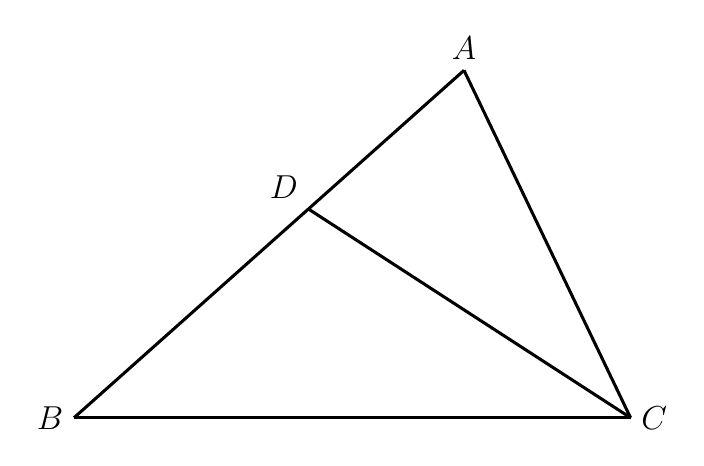
\begin{tikzpicture}[line join=round, line width=1.1pt,
  every node/.style={font=\fontsize{12}{14.4}\selectfont}]
\coordinate (A) at (1.411,2.061);
\coordinate (B) at (-3.542,-2.351);
\coordinate (C) at (3.526,-2.351);
\coordinate (D) at (-0.565,0.300);




\draw (B) -- (C);


\draw (C) -- (A);


\draw (A) -- (D) -- (B);


\draw (C) -- (D);


\node[above] at (A) {$A$};
\node[left] at (B) {$B$};
\node[right] at (C) {$C$};
\node[above left] at (D) {$D$};
\end{tikzpicture}
\end{document}